\subsubsection*{Связь метрического пространства с топологическим}

\begin{theorem} (Двойственность открытых и замкнутых множеств)
	Пусть $(X, \rho)$ --- метрическое пространство. Тогда подмножество $G \subseteq X$ является открытым тогда и только тогда, когда $F := X \bs G$ является замкнутым.
\end{theorem}

\begin{proof}~
	\begin{itemize}
		\item[$\Ra$] Рассмотрим $x \in \cl F$. Если так оказалось, что $x \in G \cap \cl F$, то существует шар $B(x, r) \subseteq G$, и, следовательно, это противоречит исходному факту о принадлежности $x$ замыканию $F$. Таким образом, остаётся лишь вариант $x \in F \cap \cl F$, то есть $F = \cl F$.
		
		\item[$\La$] Рассмотрим $x \in G$. Это же означает, что $x \notin F = \cl F$, то есть $x$ --- не точка прикосновения $F$:
		\[
			\exists r > 0 \such B(x, r) \cap F = \emptyset
		\]
		Так как $F = X \bs G$, то $B(x, r) \subseteq G$, а значит $x \in \Int G$, что и требовалось доказать.
	\end{itemize}
\end{proof}

\begin{theorem}
	Пусть $(X, \rho)$ --- метрическое пространство, $\{G_\alpha\}_{\alpha \in \gA}$ --- семейство открытых множеств, а $\{F_\beta\}_{\beta \in \gM}$ --- семейство замкнутых множеств. Тогда:
	\begin{enumerate}
		\item $\forall \gN \subseteq \gA\ \bigcup_{\alpha \in \gN} G_\alpha$ --- открытое множество
		
		\item $\forall \gZ \subseteq \gA, |\gZ| < \infty\ \bigcap_{\alpha \in \gZ} G_\alpha$ --- открытое множество
		
		\item $\forall \gN \subseteq \gM\ \bigcap_{\beta \in \gN} F_\beta$ --- замкнутое множество
		
		\item $\forall \gZ \subseteq \gM, |\gZ| < \infty\ \bigcup_{\beta \in \gZ} F_\beta$ --- замкнутое множество
	\end{enumerate}
\end{theorem}

\begin{proof}
	Достаточно доказать утверждения для открытых множеств, потому что дальше мы используем правила де Моргана и получаем оставшиеся утверждения просто через дополнения. Итак, приступим:
	\begin{enumerate}
		\item Рассмотрим $x \in \bigcup_{\alpha \in \gN} G_\alpha$. Тогда должен существовать $\alpha_0 \in \gN$, при котором этот $x$ был включен в объедиение. Стало быть, $x \in G_{\alpha_0}$, а раз $G_{\alpha_0}$ --- открытое множество, то $\exists B(x, r) \subseteq G_{\alpha_0} \subseteq \bigcup_{\alpha \in \gN} G_\alpha$, что и требовалось.
		
		\item Пусть $x \in \bigcap_{\alpha \in \gZ} G_\alpha$. Тогда этот $x$ был включен в каждое $G_\alpha$, причём в каждом из них есть свой радиус шара $r_\alpha > 0$ с центром в $x$, что $B(x, r_\alpha) \subseteq G_\alpha$. Так как мы рассмотрели конечное пересечение открытых множеств, то, взяв $r = \min_{\alpha \in \gZ} r_\alpha$, мы нашли радиус шара, включённого во все $G_\alpha$, а значит и в их пересечение.
	\end{enumerate}
\end{proof}

\begin{corollary}
	Любое метрическое пространство является топологическим, чья топология состоит из всех открытых множеств (по независимому определению конкретно в метрических пространствах).
\end{corollary}

\begin{example}
	Покажем, что существует счётное объединение замкнутых множеств, которое не является само по себе замкнутым. Достаточно рассмотреть числовую прямую и последовательность вложенных расширяющихся отрезков, которая пытается достичь другого отрезка. Например, зададим такую последовательность так:
	\[
		\forall n \in \N\ \ [a_n; b_n] = \sbr{1 + \frac{1}{n}; 4 - \frac{1}{n}}
	\]
	Казалось бы, это последовательность должна сходиться к $[1; 4]$, но на деле предел --- это интервал $(1; 4)$! Он тривиально не является замкнутым множеством за счёт своих крайних точек.
\end{example}

\begin{exercise}
	Топологическое проcтранство основных функций $D$ не является метризуемым
\end{exercise}

\begin{lemma}
	Пусть $(X, \rho)$ --- метрическое пространство, $M_{1, 2} \subseteq X$. Если $M_1 \subseteq M_2$, то и $\Int M_1 \subseteq \Int M_2$.
\end{lemma}

\begin{proof}
	Факт, на самом деле, очевидный. Если $x \in \Int M_1$, то какой-то шар с центром в этой точке включен в $M_1 \subseteq M_2$, то есть $x \in \Int M_2$.
\end{proof}

\begin{lemma}
	Пусть $(X, \rho)$ --- метрическое пространство, $M_{1, 2} \subseteq X$. Если $M_1 \subseteq M_2$, то и $\cl M_1 \subseteq \cl M_2$.
\end{lemma}

\begin{proof}
	Совсем тривиально, что точка прикосновения $M_1$ является точкой прикосновения $M_2 \supseteq M_1$.
\end{proof}

\begin{theorem}
	Пусть $(X, \rho)$ --- метрическое пространство. Тогда:
	\begin{enumerate}
		\item Открытый шар $B(x, r)$ является открытым множеством
		
		\item Для любого множества $M \subseteq X$ верно, что $\Int M$ --- открытое множество, причём наибольшее из тех, что вложены в $M$
		
		\item Для любого множества $M \subseteq X$ верно, что $\cl M$ --- замкнутое множество, причём наименьшее из тех, что содержат $M$.
		
		\item Замкнутый шар $\ole{B}(x, r)$ является замкнутым множеством
	\end{enumerate}
\end{theorem}

\begin{proof}~
	\begin{enumerate}
		\item Рассуждение довольно геометрическое. Если $y \in B(x, r)$, то по определению $y$ не лежит на границе шара, значит есть некоторое расстояние до неё и мы можем найти достаточно малый шарик, который тоже находится в $B(x, r)$. Если формально, то $\rho(x, y) < r$ и до границы у нас расстояние $l = r - \rho(x, y)$. Значит, можно рассмотреть шар $B(y, l / 2)$. Покажем, что любая точка в нём действительно остаётся в шаре $B(x, r)$:
		\begin{multline*}
			\forall z \in B(y, l / 2)\ \rho(z, y) < \frac{l}{2} \Ra
			\\
			\rho(x, z) \le \rho(x, y) + \rho(y, z) < \rho(x, y) + \frac{r - \rho(x, y)}{2} = \frac{r + \rho(x, y)}{2} < r
		\end{multline*}
		
		\item Настало время воспользоваться леммой для внутренностей. Если $x \in \Int M$, то по определению $\exists r > 0 \such B(x, r) \subseteq M$. Применив к этим множествам лемму, имеем $B(x, r) = \Int B(x, r) \subseteq \Int M$, что и требовалось показать.
		
		\item Заметим тривиальную \textit{микродвойственность}: точка $x \in X$ не лежит в замыкании $M$ тогда и только тогда, когда она лежит во внутренности $X \bs M$. Этот факт позволяет заявить, что $\cl M \sqcup \Int (X \bs M) = X$, а так как $\Int (X \bs M)$ по доказанному является открытым множеством, то в силу теоремы о двойственности мы тривиально имеем требуемое.
		
		\item Любая точка множества изначально лежит в его замыкании. Остаётся показать, что если $\rho(x, y) > r$, то такая точка не лежит в замыкании, то есть находится во внутренности дополнения к шару. Это тривиально, делается точно так же, как и в первом пункте.
	\end{enumerate}
\end{proof}

\begin{proposition}
	Пусть $(X, \rho)$ --- метрическое пространство. Всегда верно, что \\ $\ole{B(x, r)} \subseteq \ole{B}(x, r)$, но равенство выполнено не всегда.
\end{proposition}

\begin{proof}
	Для доказательства вложения достаточно заметить, что точки на расстоянии $l > r$ не могут быть точками прикосновения $B(x, r)$, ибо можно рассмотреть шар радиуса $(l - r) / 2$, который не будет пересекать $B(x, r)$, а значит остаётся лишь вариант $\le r$, который по определению соответствует $\ole{B}(x, r)$.
	
	\textcolor{red}{Контрпример нужно искать среди дискретных метрик, возможно на манхэттенской...}
\end{proof}

\begin{definition}
	Пусть $X, Y$ --- топологические пространства, $f \colon X \to Y$. Тогда $f$ называется \textit{непрерывной в точке $x_0 \in X$}, если выполнено утверждение:
	\[
		\forall\ V(f(x_0)) \in \Tau_Y\ \exists U(x_0) \in \Tau_X \such f(U(x_0)) \subseteq V
	\]
\end{definition}

\begin{figure}[h]
	\centering
	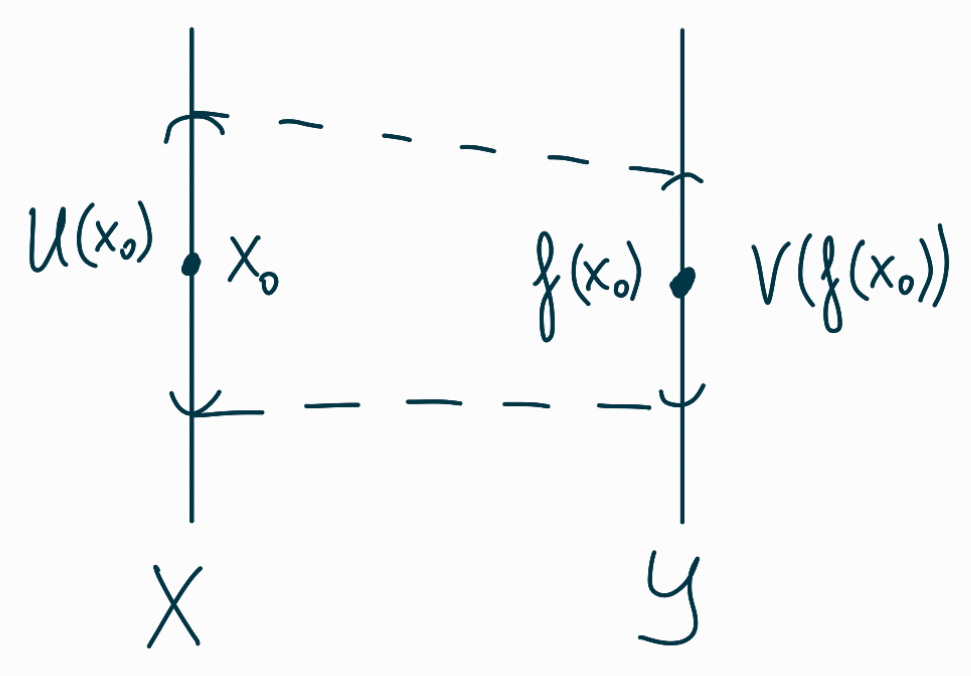
\includegraphics[width=0.4\textwidth]{images/1pic.png}
\end{figure}

\begin{definition}
	Пусть $X, Y$ --- топологические пространства, $f \colon X \to Y$ называется \textit{непрерывной}, если для любой точки $x \in X$ верно, что $f$ непрерывна в точке $x$.
\end{definition}

\begin{theorem}
	Пусть $X, Y$ --- топологическое пространство, $f \colon X \to Y$. Тогда следующие свойства функции эквивалентны:
	\begin{enumerate}
		\item $f$ непрерывна
		
		\item $\forall G \in \Tau_Y\ f^{-1}(G) \in \Tau_X$
		
		\item $\forall F \subseteq Y$ --- замкнутое множество, тогда $f^{-1}(F) \subseteq X$ --- тоже замкнутое
	\end{enumerate}
\end{theorem}

\begin{proof}
	\item $2 \Ra 1$ Тривиально
	
	\item $1 \Ra 2$ Рассмотрим $G \in \Tau_Y$ и соответствующий прообраз $f^{-1}(G)$. По определению это такое подмножество $X$:
	\[
		f^{-1}(G) = \{x \in X \colon f(x) \in G\}
	\]
	Покажем, что у каждой точки $x \in f^{-1}(G)$ есть некоторая окрестность $U(x) \in \Tau_X$, которая находится тоже в $f^{-1}(G)$. Действительно, если рассмотреть $f(x) \in G$, то по тому, что $G$ является окрестностью $f(x)$ и $f$ непрерывна, должна существовать окрестность $U(x) \in \Tau_X$ такая, что $f(U(x)) \subseteq G$, а это эквивалентно как раз требованию $U(x) \subseteq f^{-1}(G)$. Осталось заметить, что прообраз $G$ можно представить через объединение таких окрестностей:
	\[
		\ps{f^{-1}(G) = \bigcup_{x \in f^{-1}(G)} U(x),\ U(x) \in \Tau_X} \Ra f^{-1}(G) \in \Tau_X
	\]
	
	\item $2 \Lra 3$ Прообраз сохраняет все стандартные операции над множествами, поэтому эквивалентность тривиальна за счёт двойственности открытых и замкнутых множеств.
\end{proof}